% !TeX root = ../tfg.tex
% !TeX encoding = utf8

\chapter{Post-análisis de resultados con técnicas de explicabilidad} \label{chap:explicabilidad}
La explicabilidad, en el contexto de la inteligencia artificial (IA), es un concepto ético que sirve para referirse a la reducción de la opacidad (falta de transparencia) de los sistemas de IA. Su objetivo principal es aumentar la comprensión de cómo estos sistemas, particularmente aquellos con modelos de \textit{caja negra} (altamente complejos e ininteligibles para los usuarios humanos), llegan a sus predicciones o recomendaciones \parencite{ursin2023levels}.

Se considera fundamental que los modelos de IA, especialmente en aplicaciones médicas, sean explicables para que los usuarios puedan entender cómo la tecnología genera sus resultados \parencite{hildt2025role}. Un sistema de IA se considera explicable cuando es explicable e interpretable, lo que lo hace más transparente y, por lo tanto, más responsable para la toma de decisiones, la supervisión humana y las decisiones justificables.

La discusión sobre la explicabilidad en la IA a menudo se complica por la existencia de términos similares que no siempre están bien definidos o se usan indistintamente. Sin embargo, los expertos distinguen varias nociones que contribuyen a la explicabilidad general \parencite{adams2023defending}:

\begin{itemize}
    \item Transparencia (Transparency): se refiere al nivel de accesibilidad a los datos o al modelo. Un sistema de IA transparente tiene un proceso de generación de resultados no opaco donde el papel de los componentes internos, los paradigmas aprendidos y el comportamiento general del modelo son conocidos y pueden ser simulados por un usuario humano.
    \item Inteligibilidad (Intelligibility): se describe como la capacidad de un algoritmo de aprendizaje para representar su conocimiento aprendido de una manera comprensible para el ser humano. En un sentido más amplio, la inteligibilidad busca responder a la pregunta: \textit{¿Cómo funcionan los sistemas de IA en general?}. Implica entender las partes del modelo (entrada, parámetro, cálculo) y cómo aprenden de los datos de entrenamiento para generar resultados.
    \item Interpretabilidad (Interpretability): se refiere al grado en que un ser humano puede predecir el resultado de un modelo al comprender su funcionamiento interno. Se centra en cómo funciona un sistema de IA específico. Es la capacidad de traducir, exponer y comentar el proceso de generación de resultados de uno o múltiples sistemas de ML, haciendo que el proceso general sea comprensible para un ser humano. La interpretabilidad puede ser global (explicar el comportamiento del sistema para un conjunto de entradas) o local (explicar el resultado para una sola entrada).
    \item  Explicabilidad (Explainability): se refiere a la reducción de la opacidad de los sistemas de inteligencia artificial (IA), permitiendo a los usuarios comprender cómo la tecnología llega a sus predicciones o recomendaciones. Su propósito principal es responder a la pregunta fundamental: \textit{¿Por qué el sistema de IA proporcionó una salida específica?}.
\end{itemize}

La explicabilidad es fundamental en la medicina y la atención médica por varias razones:
\begin{itemize}
    \item Confianza y aceptación: ayuda a generar confianza en las herramientas de IA y facilita su aceptación por parte de los profesionales médicos y los pacientes.
    \item Toma de decisiones y autonomía: permite a los usuarios humanos, como médicos y pacientes, evaluar los resultados de la IA y utilizarlos como una \textit{segunda opinión} que apoya la toma de decisiones clínicas. 
    \item Responsabilidad: es esencial para la responsabilidad moral y legal de los profesionales médicos. No sería justo responsabilizarlos por decisiones basadas en la IA de \textit{caja negra} si no pueden entender su funcionamiento.
    \item Detección de sesgos y calidad de la IA: ayuda a los desarrolladores y clínicos a verificar si la tecnología funciona como se espera, basándose en los factores relevantes para su resultado, lo que puede ayudar a evitar errores y sesgos algorítmicos.
    \item Relaciones médico-paciente y consentimiento Informado: la explicabilidad apoya la comunicación médico-paciente significativa, la participación del paciente y la toma de decisiones compartida, permitiendo a los clínicos y pacientes reflexionar colaborativamente sobre el resultado de la IA y considerar las perspectivas y preferencias del paciente. Sin suficiente información o comprensión sobre las herramientas de IA, la participación del paciente en la toma de decisiones médicas y su autonomía se ven obstaculizadas.
\end{itemize}


En el contexto de este trabajo, la explicabilidad es especialmente importante porque estamos desarrollando un modelo de clasificación médica que predice la presencia de complicaciones tras biopsias pulmonares. Dada la naturaleza crítica de estas decisiones clínicas, no basta con obtener una predicción correcta: es fundamental entender qué partes del volumen pulmonar o qué patrones en la imagen han llevado al modelo a su conclusión. La explicabilidad permite así verificar que el modelo toma decisiones basadas en características clínicas relevantes y no en correlaciones insignificantes. Además, ayuda a generar confianza en la herramienta por parte de radiólogos y médicos, permitiéndoles integrar la predicción de la IA como una segunda opinión informada, siempre que complemente su propio juicio clínico y sea la última palabra la del médico.

\section{Análisis explicativo de los modelos 3D}
En esta sección buscamos intentar extraer conlusiones relevantes a cerca de qué aspectos de la imagen se han tenido en cuenta en los modelos 3D para la toma de las decisiones. Para ello, se han probado dos técnicas diferentes de explocabilidad post-hoc: Grad-Cam y SHAP. 

\subsection{Grad-Cam}
Grad-CAM (Gradient-weighted Class Activation Mapping) es un método de análisis de sensibilidad basado en gradientes que se utiliza principalmente para visualizar modelos de clasificación y generar mapas de calor interpretables \parencite{wang2023grad}.
Estos mapas de calor muestran la contribución e importancia de los píxeles de entrada a los resultados de una tarea de clasificación \parencite{xiao2021visualization}.

Más detalladamente, este método proporciona explicaciones visuales de las decisiones tomadas por redes profundas. Además, ayuda a entender cómo los modelos de inteligencia artificial (IA) llegan a sus decisiones, resaltando las regiones de una imagen que son más importantes para una predicción particular. Esto es crucial porque los modelos de IA a menudo se consideran \textit{cajas negras} debido a la dificultad para comprender su funcionamiento interno. Incluso, en aplicaciones críticas como el diagnóstico médico, nuestro caso, Grad-CAM puede explicar la decisión del modelo, lo que ayuda a generar confianza en su utilización. 

A lo largo de este trabajo, esta técnica también resultó útil para analizar si el modelo realmente centraba su atención en regiones relevantes. Su aplicación puso de manifiesto la necesidad de incorporar la segmentación pulmonar, dado que sin ella el modelo tendía a enfocarse en zonas externas al pulmón. Además, nos permitió identificar que era conveniente reducir el tamaño de los volúmenes de entrada, ya que en resoluciones mayores el modelo se concentraba en detalles excesivamente pequeños y clínicamente irrelevantes.

En todo momento, los mapas de activación generados mediante Grad-CAM fueron revisados y validados conjuntamente con médicos del Hospital San Cecilio con el que colaboramos, asegurando que las explicaciones proporcionadas por el modelo resultaran clínicamente coherentes y aportaran interpretaciones con sentido desde el punto de vista diagnóstico.

A continuación, se incluyen cuatro ejemplos obtenidos del propio dataset con el modelo base 3D, seleccionados para ilustrar distintos escenarios: dos predicciones correctas (una de cada clase) y dos predicciones incorrectas (una de cada clase), mostrando distintos slices relevantes para el análisis con Grad-CAM.

En el caso de la predicción correcta para la clase sin complicación (véase la Figura \ref{fig:label0-correcta}), se observa que el Grad-CAM resalta regiones relativamente amplias y distribuidas en la periferia del pulmón. Esto sugiere que el modelo explora múltiples áreas donde típicamente podrían aparecer hallazgos patológicos, verificando de manera global la ausencia de signos relevantes. Al no encontrar ningún indicio que indiquen lesiones, el modelo refuerza su predicción de sin complicación, demostrando un patrón de atención coherente con la validación clínica.

En el otro caso de predicción correcta que observamos en la Figura \ref{fig:label1-correcta}, pero para la clase con complicación (en este ejemplo, la instancia real es de hemorragia leve), se observa que el Grad-CAM destaca zonas más localizadas dentro del pulmón. Las activaciones se concentran en regiones más pequeñas y bien definidas, en particular, en las arterias bronquiales. Según la valoración clínica, esto tiene sentido, ya que la hemorragia pulmonar puede manifestarse precisamente en relación con estas estructuras vasculares. El modelo parece, por tanto, centrar su atención en áreas de interés donde podrían aparecer signos de hemorragia, lo que refuerza la interpretación clínica de la predicción y la coherencia de la explicación generada por Grad-CAM.

En el caso de las predicciones incorrectas para ambas clases (Figuras \ref{fig:label0-incorrecta} y\ref{fig:label1-incorrecta}), se observa que las activaciones del Grad-CAM tienden a concentrarse en el borde del pulmón, en lugar de en regiones interiores donde se esperaría encontrar signos patológicos relevantes. Este patrón de atención resulta poco coherente desde el punto de vista clínico, ya que no hay hallazgos significativos en esas regiones periféricas. Es posible que este comportamiento esté influido por imperfecciones en la segmentación pulmonar, que pueden inducir al modelo a aprender patrones no deseados en los contornos. 

En este sentido, la explicabilidad proporcionada por Grad-CAM resulta fundamental para analizar y comprender los fallos del modelo, ayudando a identificar las causas de errores de predicción y ofreciendo ideas para mejorar la calidad del preprocesamiento y el entrenamiento.

%----------------------------
\begin{figure}[!htbp]
\centering
\begin{subfigure}[b]{0.45\textwidth}
    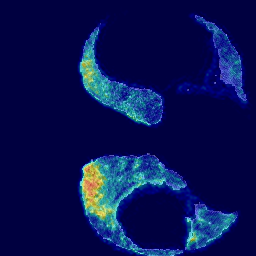
\includegraphics[width=\textwidth]{img/label0_correcto_pred0_pid65HANX_slice_21.png}
    \caption{Slice 21}
\end{subfigure}
\hfill
\begin{subfigure}[b]{0.45\textwidth}
    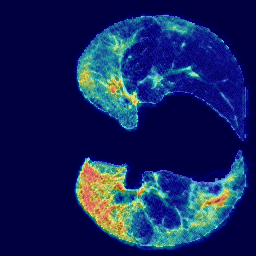
\includegraphics[width=\textwidth]{img/label0_correcto_pred0_pid65HANX_slice_42.png}
    \caption{Slice 42}
\end{subfigure}

\vspace{0.5cm}

\begin{subfigure}[b]{0.45\textwidth}
    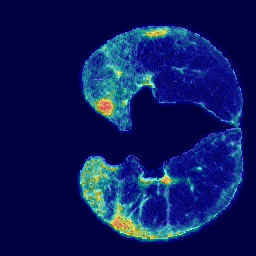
\includegraphics[width=\textwidth]{img/label0_correcto_pred0_pid65HANX_slice_63.png}
    \caption{Slice 63}
\end{subfigure}
\hfill
\begin{subfigure}[b]{0.45\textwidth}
    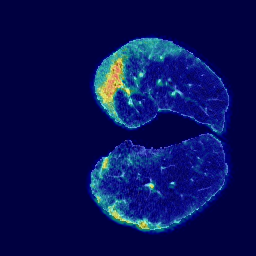
\includegraphics[width=\textwidth]{img/label0_correcto_pred0_pid65HANX_slice_84.png}
    \caption{Slice 84}
\end{subfigure}

\caption{Instancia sin complicación predicha correctamente. Elaboración propia. }
\label{fig:label0-correcta}
\end{figure}

%--------------------------------------------

\begin{figure}[!htbp]
\centering
\begin{subfigure}[b]{0.45\textwidth}
    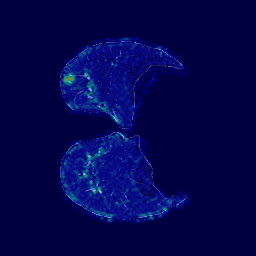
\includegraphics[width=\textwidth]{img/label1_correcto_pred1_pid95HASH_slice_42.png}
    \caption{Slice 42}
\end{subfigure}
\hfill
\begin{subfigure}[b]{0.45\textwidth}
    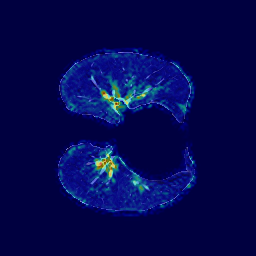
\includegraphics[width=\textwidth]{img/label1_correcto_pred1_pid95HASH_slice_63.png}
    \caption{Slice 63}
\end{subfigure}

\vspace{0.5cm}

\begin{subfigure}[b]{0.45\textwidth}
    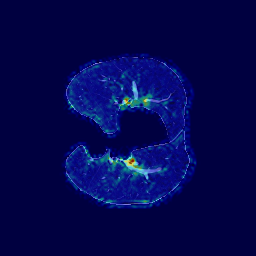
\includegraphics[width=\textwidth]{img/label1_correcto_pred1_pid95HASH_slice_84.png}
    \caption{Slice 84}
\end{subfigure}
\hfill
\begin{subfigure}[b]{0.45\textwidth}
    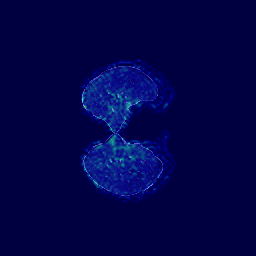
\includegraphics[width=\textwidth]{img/label1_correcto_pred1_pid95HASH_slice_105.png}
    \caption{Slice 105}
\end{subfigure}

\caption{Instancia con complicación predicha correctamente. Tipo de complicación: hemorragia leve. Elaboración propia. }
\label{fig:label1-correcta}
\end{figure}


%-------------------------------

\begin{figure}[!htbp]
\centering
\begin{subfigure}[b]{0.45\textwidth}
    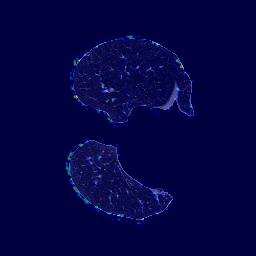
\includegraphics[width=\textwidth]{img/label0_fallo_pred1_pid32HENX_slice_42.png}
    \caption{Slice 42}
\end{subfigure}
\hfill
\begin{subfigure}[b]{0.45\textwidth}
    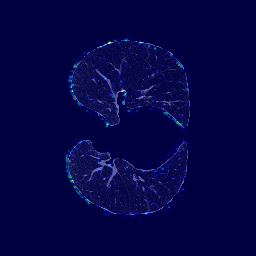
\includegraphics[width=\textwidth]{img/label0_fallo_pred1_pid32HENX_slice_63.png}
    \caption{Slice 63}
\end{subfigure}

\vspace{0.5cm}

\begin{subfigure}[b]{0.45\textwidth}
    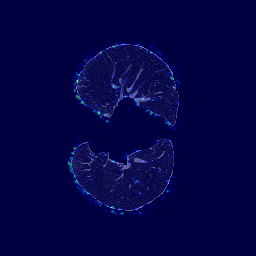
\includegraphics[width=\textwidth]{img/label0_fallo_pred1_pid32HENX_slice_84.png}
    \caption{Slice 84}
\end{subfigure}
\hfill
\begin{subfigure}[b]{0.45\textwidth}
    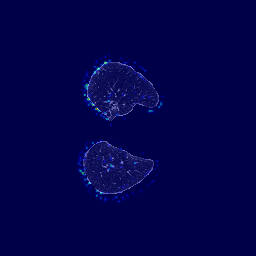
\includegraphics[width=\textwidth]{img/label0_fallo_pred1_pid32HENX_slice_105.png}
    \caption{Slice 105}
\end{subfigure}

\caption{Instancia sin complicación predicha incorrectamente. Elaboración propia. }
\label{fig:label0-incorrecta}
\end{figure}


%----------------------------

\begin{figure}[!htbp]
\centering
\begin{subfigure}[b]{0.45\textwidth}
    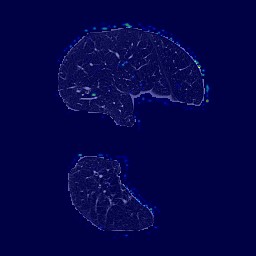
\includegraphics[width=\textwidth]{img/label1_fallo_pred0_pid87MASSN_slice_42.png}
    \caption{Slice 42}
\end{subfigure}
\hfill
\begin{subfigure}[b]{0.45\textwidth}
    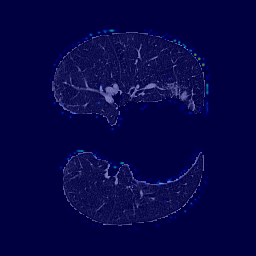
\includegraphics[width=\textwidth]{img/label1_fallo_pred0_pid87MASSN_slice_63.png}
    \caption{Slice 63}
\end{subfigure}

\vspace{0.5cm}

\begin{subfigure}[b]{0.45\textwidth}
    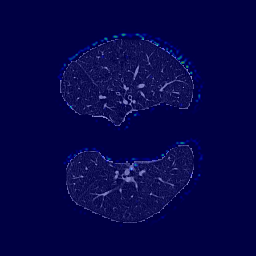
\includegraphics[width=\textwidth]{img/label1_fallo_pred0_pid87MASSN_slice_84.png}
    \caption{Slice 84}
\end{subfigure}
\hfill
\begin{subfigure}[b]{0.45\textwidth}
    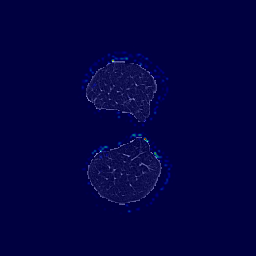
\includegraphics[width=\textwidth]{img/label1_fallo_pred0_pid87MASSN_slice_105.png}
    \caption{Slice 105}
\end{subfigure}

\caption{Instancia sin complicación predicha correctamente. Tipo de complicación: neumotórax y hemorragia. Elaboración propia. }
\label{fig:label1-incorrecta}
\end{figure}




\subsection{Shap}
Queríamos validar los resultados obtenidos con \textit{Grad-CAM} empleando una técnica de explicabilidad complementaria. La idea era comprobar si los mapas de activación generados por \textit{Grad-CAM} reflejaban realmente información significativa sobre el modelo o si, por el contrario, las inconsistencias detectadas se debían a limitaciones de la propia técnica de visualización. Este contraste nos permitiría distinguir si los problemas observados eran debidos a un mal entrenamiento del modelo o a la herramienta de explicabilidad en sí.

Para ello, realizamos una prueba con SHAP (\textit{SHapley Additive exPlanations}), un método de interpretabilidad muy popular por su versatilidad y capacidad para explicar las predicciones de modelos de aprendizaje automático \parencite{ponce2024practical}. Su objetivo es mejorar la transparencia y la confianza en los sistemas de IA, permitiendo comprender cómo el modelo llega a sus decisiones.

SHAP se basa en la teoría de los valores de Shapley para cuantificar la contribución de cada característica a la predicción de un modelo. Para una muestra específica, el valor SHAP de una característica indica en qué medida contribuye a la diferencia entre la predicción individual de esa muestra y la predicción media del modelo.

En el ámbito de las imágenes, SHAP permite visualizar qué regiones son más influyentes para la predicción de un modelo. Dado que un solo píxel no suele ser interpretable por sí mismo, SHAP agrupa los píxeles en segmentos homogéneos llamados \textit{superpíxeles}. Estos superpíxeles se consideran las \textit{características} de entrada para el modelo explicativo de SHAP \parencite{dewi2023xai}.

Sin embargo, en nuestro caso concreto, SHAP no resultó especialmente útil, ya que su salida no era tan interpretable en volúmenes 3D. Por este motivo, tras una prueba inicial, decidimos no emplearlo de forma sistemática en los experimentos y priorizamos el análisis con \textit{Grad-CAM}, que ofrecía mapas de activación más coherentes y comprensibles para el equipo médico.


\section{Análisis explicativo de los modelos radiómicos}

\subsection{Análisis post-hoc con SHAP}

Con el objetivo de extraer conclusiones interpretables de los datos radiómicos, se ha seleccionado la versión del algoritmo \texttt{LightGBM} que mejores resultados dio al utilizar los datos radiómicos combinados con los datos clínicos, y se ha aplicado también la técnica SHAP para estimar la importancia de cada atributo en la clasificación. La experimentación se ha realizado sobre el fold de validación cruzada que mejores resultados obtuvo en test. Se ha aplicado SHAP sobre todos los pacientes de test y se han analizado sus resultados.

En la Figura \ref{fig:shap} podemos ver el análisis global que proporciona SHAP sobre las predicciones realizadas por LightGBM. Es un diagrama de enjambre en el que se muestra el ranking de características más influyentes. En el eje Y se observan las características radiómicas y clínicas ordenadas por importancia, mientras que en el eje X se observa el valor SHAP, o el impacto en la predicción del modelo. Cada punto del diagrama representa a un paciente, y el color representa el valor del atributo en cuestión.

Por ejemplo, podemos observar que el atributo con mayor impacto global en la predicción es una característica radiómica de la matriz GLSZM calculada sobre la imagen mediante una transformación wavelet-HLL. Vemos que hay hasta 4 pacientes que se destacan con un impacto muy alto en la predicción positiva. El color azul además indica que los valores de este atributo en estos pacientes es bajo. Esto nos da la idea de que valores bajos de esa característica radiómica pueden contribuir a una predicción positiva de complicación. En la siguiente característica, \texttt{ngtdm\_Busyness} bajo la transformación logarítmica, observamos también algo interesante. En la frontera de impacto (el valor shap 0), podemos ver que hacia la derecha todos los valores presentan un valor alto del atributo, mientras que a la derecha todos presentan un valor bajo. Esto se podría interpretar como que este atributo es muy influyente en la toma de decisiones, ya que proporciona una predicción positiva siempre que es alto y una predicción negativa siempre que es bajo. En el tercer atributo sucede al contrario, indicando que valores bajos pueden contribuir a la predicción positiva y valores bajos a la negativa. En general, la información de la Figura \ref{fig:shap} puede ser de gran interés clínico, ya que se puede combinar con el conocimiento experto de los médicos para tratar de extraer conclusiones relevantes sobre las características relevantes y su importancia en las predicciones.

Otro aspecto a destacar sobre la Figura \ref{fig:shap} a nivel global es qué tipos de atributos son los más destacados. Podemos ver que predominan las transformaciones wavelet, variando el tipo de filtro empleado en cada eje. En general, las características radiómicas transformadas dominan la gráfica, apareciendo características originales en 2 de las 20 características más destacadas. Esto nos puede indicar que, efectivamente, el uso de características radiómicas obtenidas a partir de las transformaciones de la imagen introduce información relevante en el problema de clasificación. Por otra parte, podemos ver que no llega a verse ninguna característica clínica, pese a que en este modelo se utilizaron características radiómicas y clínicas conjuntamente. Esto nos indica que, para el modelo LightGBM entrenado, los datos clínicos no parecen haber sido especialmente relevantes para determinar una posible complicación o no.

\begin{figure}
    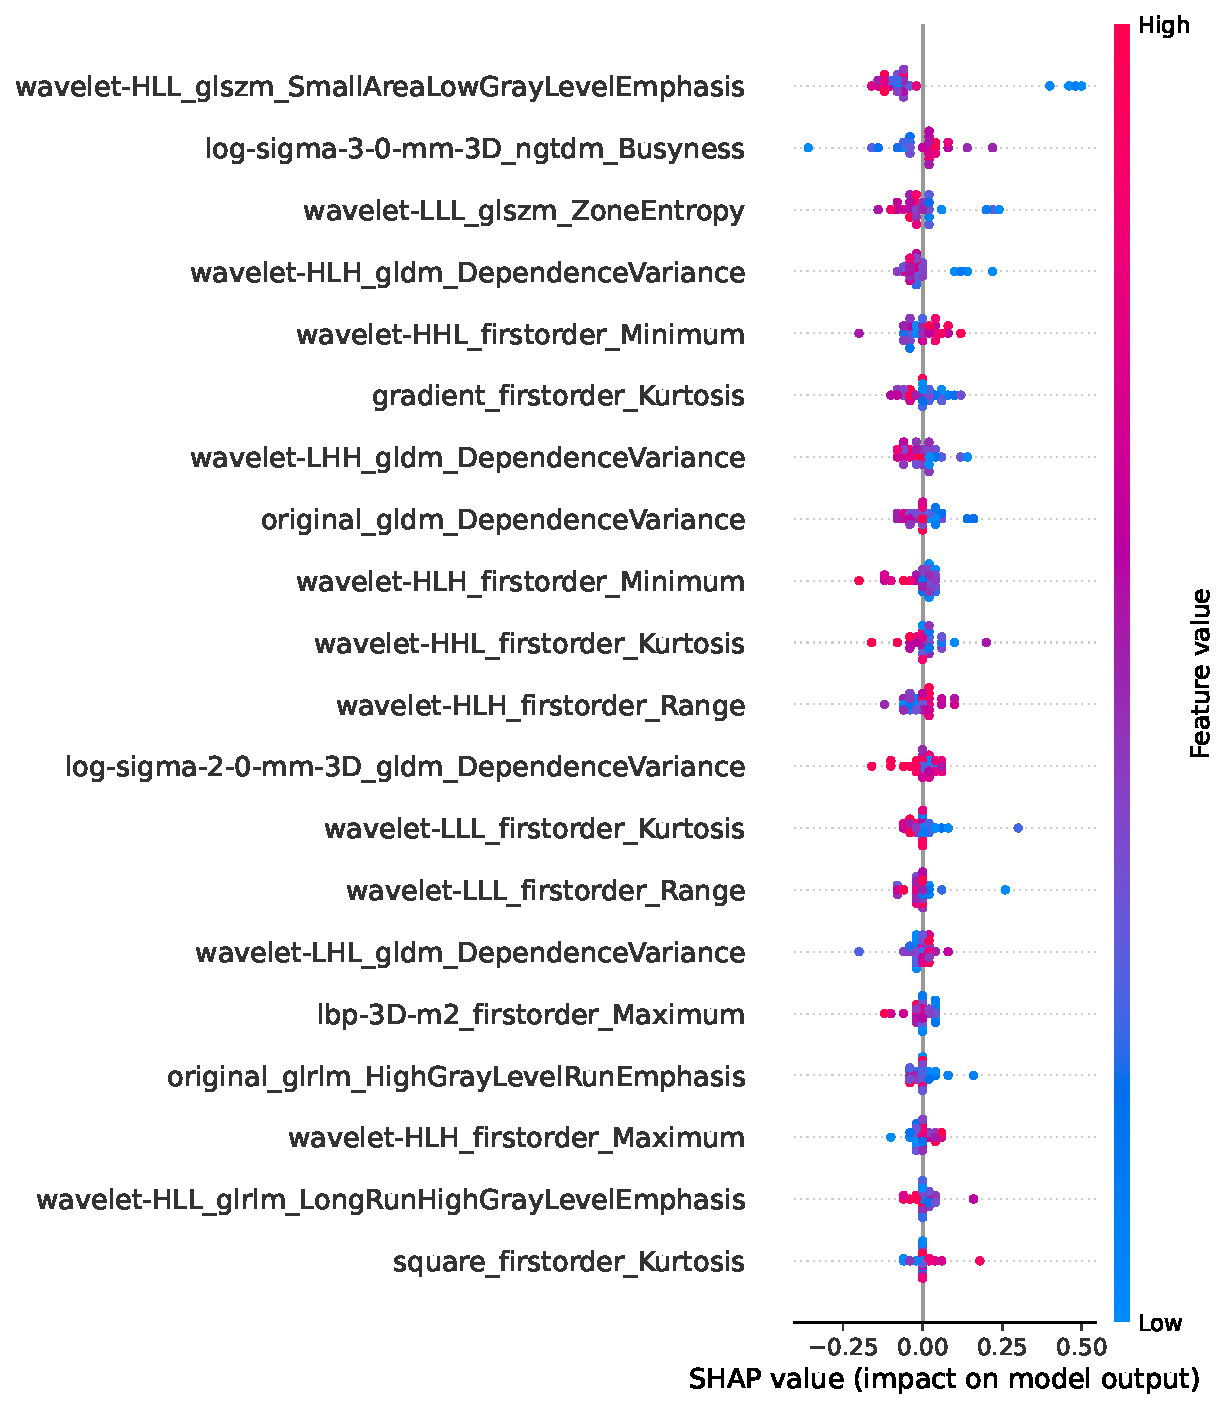
\includegraphics[width=\textwidth]{shap_summary_plot_lighbmg_extended.pdf} \caption{Diagrama resumen de las características más influyentes en la predicción de LightGBM según SHAP.}\label{fig:shap}
    
\end{figure}

Para concluir el análisis de SHAP vamos a realizar un análisis a nivel de paciente. En las Figuras \ref{fig:shap_tn}, \ref{fig:shap_tp} y \ref{fig:shap_f} se muestran, respectivamente, los análisis de SHAP sobre los pacientes predichos correctamente como positivos, como negativos, y los pacientes en los que el algoritmo se ha equivocado. Estas imágenes son gráficos en cascada en los que se representan los atributos más relevantes para cada paciente y el empuje que realizan hacia una predicción positiva (rojo) o negativa (azul). Se parte desde la probabilidad media de predicción de complicación obtenida por el modelo ($E[f(X)] = 0.4$), y los distintos atributos van empujando en una dirección u otra, hasta llegar a la probabilidad final de complicación, que alcanza el 1 en todos los pacientes predichos como positivos y 0 en los negativos. También podemos observar el valor de entrada de cada atributo.

Podemos ver que las características más destacadas del análisis global, como la GLSZM de la transformada wavelet o el \texttt{ngtdm\_Busyness} de la transformada logarítmica, están presentes también individualmente en la mayoría de pacientes. Podemos observar sus valores y confirmar que en las predicciones positivas están con valores bajos y altos, respectivamente, y al revés en las predicciones positivas. También es interesante observar que, como es de esperar, en las predicciones positivas predominan los atributos que empujan hacia la clase positiva (en rojo), mientras que en las negativas predominan los atributos que empujan hacia la negativa (azul).Sin embargo, siempre podemos identificar ciertos atributos que empujan hacia la clase contraria. Estos atributos pueden entenderse como señales de alerta: aunque el modelo ha tomado una decisión concreta, ha percibido cierta información que puede contener evidencias de pertenencia a la clase contraria. Estas características, pueden analizarse desde el punto de vista médico para corroborar o poner en duda las decisiones tomadas por el modelo, y así actuar convenientemente. Podemos observar además que muchas veces los patrones de alerta son comunes en todos los pacientes. Por ejemplo, en muchos pacientes, podemos ver atributos de primer orden como la curtosis, el mínimo o el máximo suelen empujar hacia la clase contraria a la predicha.

Por último, si nos fijamos en los falsos positivos y falsos negativos, a priori no se observa ningún patrón diferente con respecto a las predicciones correctas. Los atributos siguen empujando en su mayoría hacia la clase predicha, con ciertas excepciones, aunque en estos casos observamos que entre las señales de alerta no aparecen tanto curtosis, máximos y mínimos. Lo que sí que vemos es que las características predominantes a nivel global son dominantes en estos ejemplos y, posiblemente, son determinantes en la toma de la decisión errónea por parte del modelo.





% ============================================
% PRIMERA PÁGINA - VERDADEROS NEGATIVOS
% ============================================
\begin{figure}[p]
    \centering
    

    \medskip
    \foreach \i in {0,4,5,6,7,8,9,13,15,16,17,20,22}{
        \begin{subfigure}[b]{0.45\textwidth}
            \includegraphics[width=\linewidth]{patient_\i_label_0_pred_0.pdf}
        \end{subfigure}
    }

    \caption{Análisis de SHAP de los pacientes clasificados correctamente como negativos.}\label{fig:shap_tn}

\end{figure}


% ============================================
% SEGUNDA PÁGINA - VERDADEROS POSITIVOS
% ============================================
\begin{figure}[p]
    \centering

    \medskip
    \foreach \i in {2,3,10,14,18,19,21,23,24}{
        \begin{subfigure}[b]{0.47\textwidth}
            \includegraphics[width=\linewidth]{patient_\i_label_1_pred_1.pdf}
        \end{subfigure}
    }
    \caption{Análisis de SHAP de los pacientes clasificados correctamente como positivos.}\label{fig:shap_tp}
\end{figure}

\clearpage

% ============================================
% TERCERA PÁGINA - FALSOS POSITIVOS Y FALSOS NEGATIVOS
% ============================================
\begin{figure}[p]
    \centering
    % --- Falsos Positivos ---
    \vspace{0.5cm}
    \textbf{Falso Positivo}

    \medskip
    \foreach \i in {1}{
        \begin{subfigure}[b]{0.47\textwidth}
            \includegraphics[width=\linewidth]{patient_\i_label_0_pred_1.pdf}
        \end{subfigure}
    }

    % --- Falsos Negativos ---
    \vspace{0.8cm}
    \textbf{Falsos Negativos}

    \medskip
    \foreach \i in {11,12}{
        \begin{subfigure}[b]{0.47\textwidth}
            \includegraphics[width=\linewidth]{patient_\i_label_1_pred_0.pdf}
        \end{subfigure}
    }

    \caption{Análisis de SHAP de los pacientes clasificados incorrectamente.}\label{fig:shap_f}

\end{figure}

\subsection{Discusión de aproximaciones alternativas}

En la experimentación con datos radiómicos se probó a utilizar árboles de decisión, algoritmos que por naturaleza son explicables. Sin embargo, no obtuvieron resultados demasiado buenos. Sí hubo una combinación razonable que alcanzó un 0.67 de F1 y 0.7 de G-Mean, aunque este fue aplicado sobre un preprocesamiento con PCA al 95 \% de la varianza. Por tanto, la información que obtiene el árbol de decisión es a partir de dichas componentes principales, en lugar de las características radiómicas. Por tanto, para poder hacer un análisis explicativo razonable habría que analizar en primer lugar dichas componentes principales y ver qué atributos se combinan mayoritariamente en cada componente, lo cual tiene una complejidad elevada. En la Figura \ref{fig:expl_arbol} se muestra la secuencia de divisiones realizadas por el árbol de decisión aprendido para determinar la clase a partir de las componentes principales.

\begin{figure}
    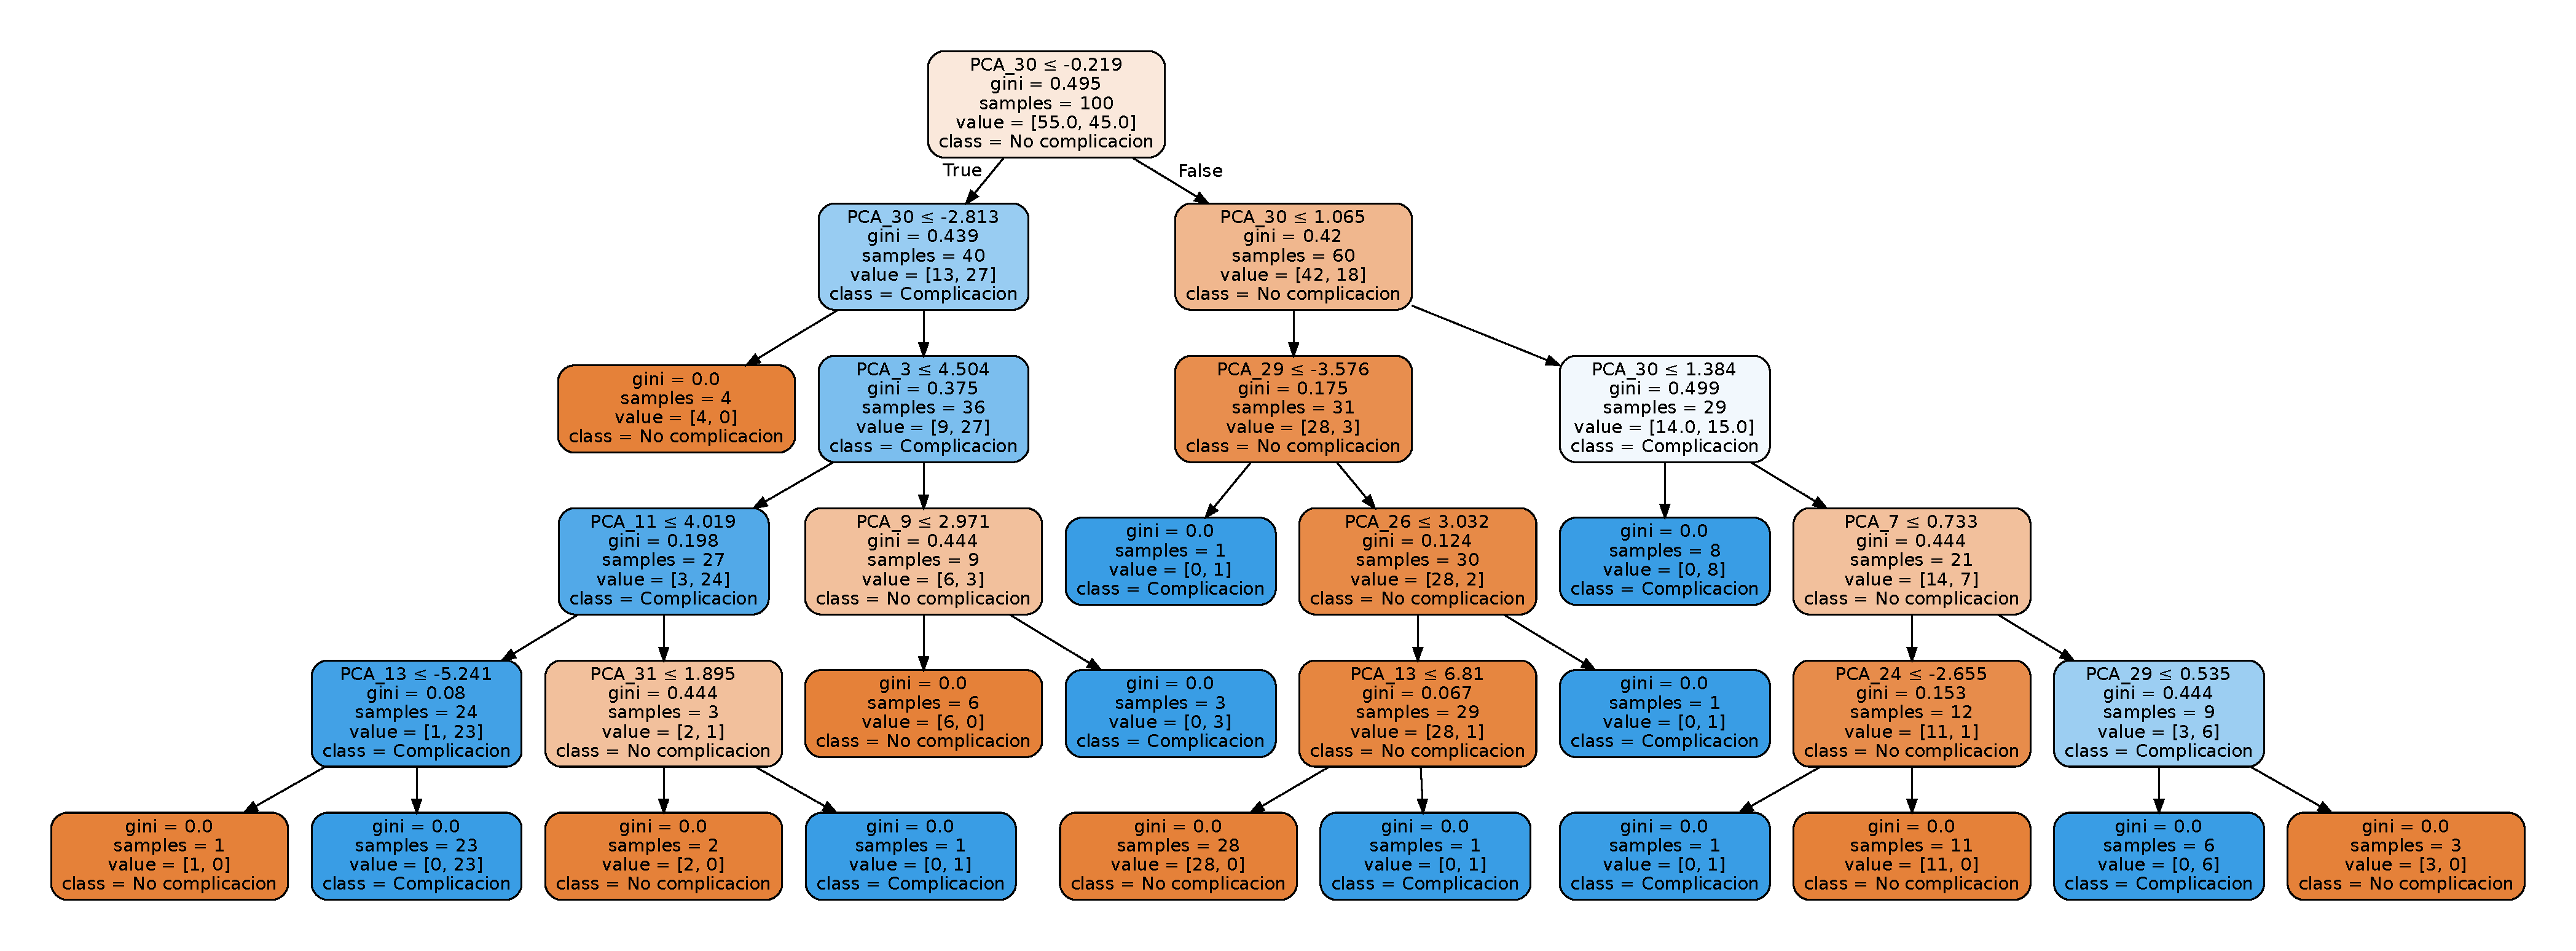
\includegraphics[width=\textwidth]{arbol_decision.pdf} \caption{Análisis de la toma de decisiones mejor modelo de árbol de decisión obtenido en función de las componentes principales extraídas.}\label{fig:expl_arbol}
\end{figure}

Por último, dada la especial relevancia que han tenido los algoritmos basados en distancias en la experimentación radiómica, es relevante comentar que en las implementaciones de $k$-NN podemos analizar los vecinos más cercanos que se han utilizado para la toma de una decisión concreta. Desde el punto de vista médico, los expertos médicos podrían en estas situaciones analizar los TC y datos clínicos de los ejemplos ya conocidos que han sido marcados como los más similares al ejemplo a predecir, y corroborar o descartar la decisión del modelo apoyándose en su juicio médico.


\endinput
%--------------------------------------------------------------------
% FIN DEL CAPÍTULO. 
%--------------------------------------------------------------------
